\documentclass[openany,12pt]{book}
\usepackage[utf8]{inputenc}
\usepackage{fontspec}
\usepackage[frenchb]{babel} % If you write in French
%\usepackage[english]{babel} % If you write in English
\usepackage{a4wide}
\usepackage{graphicx}
\graphicspath{{images/}}
\usepackage{subfig}
\usepackage{tikz}
\usepackage{float}
\usepackage{array}
\setromanfont [Ligatures={Common}, Numbers={OldStyle}, Variant=01]{Linux Libertine O}
\setmonofont[Scale=0.8]{SansSerif.ttf}
\usetikzlibrary{shapes,arrows}
\usepackage{pgfplots}
\pgfplotsset{compat=newest}
\pgfplotsset{plot coordinates/math parser=false}
\newlength\figureheight
\newlength\figurewidth
\pgfkeys{/pgf/number format/.cd,
set decimal separator={,\!},
1000 sep={\,},
}
\usepackage{ifthen}
\usepackage{ifpdf}
\ifpdf
\usepackage[pdftex]{hyperref}
\else
\usepackage{hyperref}
\fi
\usepackage{color}
\hypersetup{%
colorlinks=true,
linkcolor=black,
citecolor=black,
urlcolor=black}

\renewcommand{\baselinestretch}{1.05}
\usepackage{fancyhdr}
\pagestyle{fancy}
\fancyfoot{}
\fancyhead[LE,RO]{\bfseries\thepage}
\fancyhead[RE]{\bfseries\nouppercase{\leftmark}}
\fancyhead[LO]{\bfseries\nouppercase{\rightmark}}
\setlength{\headheight}{15pt}

\let\headruleORIG\headrule
\renewcommand{\headrule}{\color{black} \headruleORIG}
\renewcommand{\headrulewidth}{1.0pt}
\usepackage{colortbl}
\arrayrulecolor{black}

\fancypagestyle{plain}{
  \fancyhead{}
  \fancyfoot[C]{\thepage}
  \renewcommand{\headrulewidth}{0pt}
}

\makeatletter
\def\@textbottom{\vskip \z@ \@plus 1pt}
\let\@texttop\relax
\makeatother
\definecolor{niceblue}{rgb}{.149,.129,.647}
\definecolor{nicered}{rgb}{.647,.129,.149}
\definecolor{MSBlue}{rgb}{.204,.353,.541}
\definecolor{MSLightBlue}{rgb}{.31,.506,.741}
\definecolor{vert}{RGB}{11, 102, 35}

\usepackage{titlesec}
\titleformat*{\section}{\Large\bfseries\sffamily}
\titleformat*{\subsection}{\large\bfseries\sffamily}
\titleformat*{\subsubsection}{\bfseries\sffamily\color{MSBlue}}

\setcounter{secnumdepth}{4}

\titleformat{\paragraph}
{\normalfont\normalsize\bfseries}{\theparagraph}{1em}{}
\titlespacing*{\paragraph}
{0pt}{3.25ex plus 1ex minus .2ex}{1.5ex plus .2ex}

\usepackage{amsthm}
\usepackage{amssymb,amsmath,bbm}
\usepackage{array}
\usepackage{bm}
\usepackage{multirow}
\usepackage[footnote]{acronym}

\usepackage{listings}
\usepackage{color}

\definecolor{dkgreen}{rgb}{0,0.6,0}
\definecolor{gray}{rgb}{0.5,0.5,0.5}
\definecolor{mauve}{rgb}{0.58,0,0.82}

\lstset{frame=tb,
  language=Java,
  aboveskip=3mm,
  belowskip=3mm,
  showstringspaces=false,
  columns=flexible,
  basicstyle={},
  numbers=none,
  numberstyle=\tiny\color{gray},
  keywordstyle=\color{blue},
  commentstyle=\color{dkgreen},
  stringstyle=\color{mauve},
  breaklines=true,
  breakatwhitespace=true,
  tabsize=3
}
%\sloppy

\begin{document}

%%%%%%%%%%%%%%%%%%
%%% First page %%%
%%%%%%%%%%%%%%%%%%

\begin{titlepage}
\begin{center}


\includegraphics[width=0.6\textwidth]{logoNanterre.jpg}\\[1cm]

{\large Master 2 Méthodes Informatiques Appliquées à la Gestion d'Entreprise \textit{parcours Agilité des Systèmes d'Information et E-business}}\\[0.5cm]

{\large Mémoire de recherche}\\[0.5cm]

% Title
\rule{\linewidth}{0.5mm} \\[0.4cm]
{ \huge \bfseries Automatisation des tests d'acceptation à partir des exigences \\[0.4cm] }
\rule{\linewidth}{0.5mm} \\[1.5cm]

% Author and supervisor
\noindent
\begin{minipage}{0.4\textwidth}
  \begin{flushleft} \large
    \emph{Auteur :}\\
    Khaoula \textsc{ZITOUN}\\
  \end{flushleft}
\end{minipage}%
\begin{minipage}{0.4\textwidth}
  \begin{flushright} \large
    \emph{Encadrant :} \\
    Pr.~Pascal \textsc{POIZAT}\\
  \end{flushright}
\end{minipage}

\vfill

% Bottom of the page
{\large Version 1.0 du\\ \today}

\end{center}
\end{titlepage}

%%%%%%%%%%%%%%%%%%%%%%%%%%%%%
%%% Non-significant pages %%%
%%%%%%%%%%%%%%%%%%%%%%%%%%%%%

\frontmatter

\chapter*{Remerciements}

Je tiens tout d'abord à remercier le Professeur Pascal Poizat, Professeur des Universités à l'université Paris Nanterre pour ses précieux conseils pour la rédaction de ce mémoire. Je le remercie également pour le temps qu'il m'a consacré à répondre à mes interrogations.

D'autre part, je souhaite remercier Khadija Machhout, Hajer Zitoun, Sana Zitoun et Adem Maadi pour leur soutien tout au long de cette dernière année de Master.

Je remercie aussi Adil Houssni et Jean-Christophe Claye de m'avoir accordé le temps et l'espace de travail nécessaire à la rédaction de cet écrit. 

Enfin mes remerciements vont à l'équipe Europcar de Capgemini de m'avoir motivée pendant la rédaction de ce mémoire. Mention spéciale pour Sanae, Sebastien, Martin, Vincent, Nabil, Saâd, Abdoulaye et Edmond. 

\tableofcontents
\listoffigures

%%%%%%%%%%%%%%%%%%%%%%%%%%%%%%%%%%%%%%%%%%%%
%%% Content of the report and references %%%
%%%%%%%%%%%%%%%%%%%%%%%%%%%%%%%%%%%%%%%%%%%%

\mainmatter
\pagestyle{fancy}
\chapter*{Introduction}
\addcontentsline{toc}{chapter}{Introduction}
\markboth{Introduction}{Introduction}
\label{chap:introduction}
%\minitoc

Les projets informatiques sont généralement le résultat de l'implantation d'un ou des besoins exprimés. 

Depuis 1994, les résultats du rapport CHAOS du Standish Group sont mis à jour chaque année et montrent les principales raisons d’échec et de succès d’un projet au sein d’un panel représentatif d’entreprises américaines. Les différentes études montrent que les projets qui se terminent dans le temps et le budget avec un périmètre fonctionnel livré conforme au périmètre initialement défini représentent 20\%. Les projets qui se terminent en ayant respecté le temps ou le budget avec un périmètre fonctionnel livré légèrement différent  du périmètre initial représentent 50\%. Enfin les projets qui ont été abandonnés en cours de projet pour diverse raisons représentent 30\%. Il est donc à souligner que le taux d’échec des projets reste important. Par ailleurs, ce rapport montre que parmi les facteurs d'échec, 44,1\% d'entre eux sont relatifs au exigences (exigences incomplètes, manque d'implication des utilisateurs, changement sur les exigences et les spécifications). D'autre part, les facteurs de succès d'un projet relatifs aux exigences représentent 37,1\% (implication des utilisateurs, définition claire des exigences, attentes réalistes).~\cite{livre1}
Cette étude nous permet donc d’affirmer que l’implication des parties prenantes ainsi que la définition et la gestion des exigences jouent un rôle important dans l’avenir d’un projet.

L'implication des parties prenantes permet notamment de réduire l'écart qui existent entre celles-ci~\cite{article5}. En effet, un écart de communication entre les experts du domaine et les ingénieurs en logiciel a été observé~\cite{article1}, comme cela a été rapporté par des chercheurs.~\cite{article2}. Définir des exigences pour ensuite les implanter peut donc devenir périlleux. Les experts domaines, n'ayant pas forcément des compétences techniques mais métier, et les ingénieurs en logiciel ayant des compétences techniques mais n'appréhendant pas entièrement tous les domaines, il est donc nécessaire de trouver un moyen de définir les exigences tout en s'assurant que les experts puissent les rédiger et les ingénieurs les comprendre. 

D'après la définition du IEEE et du CMMi une exigence est:
  \textit{\guillemotleft  \begin{enumerate}
    \item Condition ou capacité nécessaire à un utilisateur pour résoudre un problème ou atteindre un objectif.
    \item Condition ou capacité qui doit être assurée par un produit pour satisfaire à un contrat, une norme, une spécification ou à d’autres documents imposés formellement. 
    \item Une représentation documentée de cette condition ou capacité telle que définie en 1. ou 2.
\end{enumerate}\guillemotright}

Il existe plusieurs niveaux d'exigences : les besoins des utilisateurs, les exigences métier qui sont défini à partir des besoins et les exigences produit qui traduisent la solution fonctionnelle et technique. De plus, il existe plusieurs types d'exigences : les exigences fonctionnelles, les exigences non fonctionnelles, les exigences de contrainte. Dans ce mémoire nous nous axerons sur les exigences fonctionnelles. Après avoir recueilli le besoin des utilisateur il est important de définir les exigences.L'objectif de la définition des exigences est de les exprimer de manière compréhensible par tous.~\cite{Gestion} Les exigences sont exprimées de différentes manières mais pas toujours compréhensibles par tous. Une solution à ceci problématique est l'ingénierie des domaines. Cette dernière est un élément clé pour que l'ingénierie des exigences soit efficace~\cite{article3}.

La spécification des exigences lieés au domaine nécessite un langage d'exigences propre au domaine : les Domain Specific Requirement Language (DSRL). Ces langages permettent de spécifier les exigences en terme d'abstractions de domaine d'application.~\cite{article3} Certaines approches sont génériques et sont des solutions à de nombreuses problématiques générales de certains domaines. Il arrive toutefois que ces approches ne répondent pas à des problèmes spécifiques à un domaine. Une approche spécifique fournit une bien meilleure solution pour un ensemble plus restreint de problèmes.~\cite{article4}  Les Domain Specific Model rendent la modélisation des exigences moins compliquée et réduit l'effort d'apprentissage pour les scientifiques et favorise le génie logiciel dans les projets.~\cite{article5}

\guillemotleft \textit{Le but de l'ingénierie de domaine est d'identifier, de modéliser, de construire, de cataloguer et de diffuser des artefacts qui représentent les points communs et les différences au sein d'un domaine.~\cite{livre3,article4}} \guillemotright. La modélisation de ces artefacts peuvent se faire de différentes façons : par des diagrammes UML, SysML,les DSL (Domain Specific Language), etc que nous présenterons dans la première partie de ce mémoire.

Bien qu'il existe des méthodes pour modéliser le domaine métier qui nous permettrait de définir les exigences fonctionnelles, il n'en reste pas moins que des tests d'acceptation sont nécessaires pour assurer la satisfaction du client. Ces tests sont souvent créés en fonction d'une spécification des exigences et servent à vérifier que les obligations contractuelles sont respectées.~\cite{article6} Il semble nécessaire de déterminer comment valider des exigences orientées domaine en passant par les tests. 
Il existe beaucoup de recherches et d'implantations d'outils sur des tests basés sur des modèles, la dérivation de tests à partir d'un modèle.~\cite{article7} Dans ce document nous nous intéresseront aux tests relatifs à la recette tels que les tests d'acceptation, appelés aussi tests fonctionnels. Les tests d'acceptation peuvent être spécifiés de plusieurs façons: depuis les user stories basées sur la compréhension de textes suivis jusqu'aux langages formels. Parce que l'exécution des tests d'acceptation est longue et coûteuse, il est hautement souhaitable d'automatiser ce processus. \textit{L'automatisation des tests d'acceptation donne une réponse objective lorsque les exigences fonctionnelles sont remplies.~\cite{article6}}

La définition des exigences fonctionnelles et la vérification de ces dernières jouent donc un rôle important dans la réussite d'un projet. Nous souhaitons donc dans ce mémoire répondre à la problématique suivante : 
  \textbf{comment à partir d'une spécification d'exigences générer des tests d'acceptation en mettant le domaine métier au coeur de la démarche ? }


Dans ce document nous présenterons dans une première section comment définir des exigences, quelques outils de suivi, les différentes méthodes de modélisation du domaine ainsi que les techniques de génération de tests.


\chapter{Premier chapitre}
\label{chap:premierchapitre}

\section{Une section}
Lorem ipsum dolor sit amet, consectetur adipiscing elit \cite{Roque2012,Roque2012b,Roque2012c,Roque2012d}. Sed non risus. Suspendisse lectus tortor, dignissim sit amet, adipiscing nec, ultricies sed, dolor. Cras elementum ultrices diam. Maecenas ligula massa, varius a, semper congue, euismod non, mi. Proin porttitor, orci nec nonummy molestie, enim est eleifend mi, non fermentum diam nisl sit amet erat. Duis semper. Duis arcu massa, scelerisque vitae, consequat in, pretium a, enim. Pellentesque congue. Ut in risus volutpat libero pharetra tempor. Cras vestibulum bibendum augue. Praesent egestas leo in pede. Praesent blandit odio eu enim. Pellentesque sed dui ut augue blandit sodales. Vestibulum ante ipsum primis in faucibus orci luctus et ultrices posuere cubilia Curae; Aliquam nibh. Mauris ac mauris sed pede pellentesque fermentum. Maecenas adipiscing ante non diam sodales hendrerit. Ut velit mauris, egestas sed, gravida nec, ornare ut, mi. Aenean ut orci vel massa suscipit pulvinar. Nulla sollicitudin. Fusce varius, ligula non tempus aliquam, nunc turpis ullamcorper nibh, in tempus sapien eros vitae ligula. Pellentesque rhoncus nunc et augue. Integer id felis. Curabitur aliquet pellentesque diam. Integer quis metus vitae elit lobortis egestas. Lorem ipsum dolor sit amet, consectetuer adipiscing elit. Morbi vel erat non mauris convallis vehicula. Nulla et sapien. Integer tortor tellus, aliquam faucibus, convallis id, congue eu, quam. Mauris ullamcorper felis vitae erat. Proin feugiat, augue non elementum posuere, metus purus iaculis lectus, et tristique ligula justo vitae magna. Aliquam convallis sollicitudin purus. Praesent aliquam, enim at fermentum mollis, ligula massa adipiscing nisl, ac euismod nibh nisl eu lectus. Fusce vulputate sem at sapien. Vivamus leo. Aliquam euismod libero eu enim. Nulla nec felis sed leo placerat imperdiet. Aenean suscipit nulla in justo. Suspendisse cursus rutrum augue. Nulla tincidunt tincidunt mi. Curabitur iaculis, lorem vel rhoncus faucibus, felis magna fermentum augue, et ultricies lacus lorem varius purus. Curabitur eu amet (fig. \ref{fig:une-image}). Deux citations \cite{Arapoglou2011,Roque2013c}.

\begin{figure}[htp]
  \centering
  \tikzstyle{block} = [draw, fill=blue!20, rectangle, minimum height=3em, minimum width=6em, text width=6em,text centered]
\begin{tikzpicture}[auto, node distance=3.5cm,>=latex']
\shorthandoff{:} % Evite le bug de compilation avec tikz
    % Longueurs et espacement
    \def\longabove{0.2cm}
    \def\espacement{4cm}

    % Définition des blocs
    \node [block, node distance=\espacement] (codeur) {Codeur};
    \node [block, right of=codeur, node distance=\espacement] (cbs) {CBS};
    \node [block, right of=cbs, node distance=\espacement] (modulateur) {Modulateur};
 
    % Définition des liens
    \draw [<-] (codeur) -- ++(-2,0) node[left] {$\{b_n\}$};
    \draw [->] (codeur) -- node[above=\longabove] {$\{d_n\}$} (cbs);
    \draw [->] (cbs) -- node[above=\longabove] {$\{c_k\}$} (modulateur);
    \draw [->] (modulateur) -- ++(2,0) node[right] {$s(t)$};
\end{tikzpicture}

  \caption{Exemple de diagramme TikZ.}
  \label{fig:une-image}
\end{figure}

\section{Une autre section}
Lorem ipsum dolor sit amet, consectetur adipiscing elit. Sed non risus. Suspendisse lectus tortor, dignissim sit amet, adipiscing nec, ultricies sed, dolor. Cras elementum ultrices diam. Maecenas ligula massa, varius a, semper congue, euismod non, mi. Proin porttitor, orci nec nonummy molestie, enim est eleifend mi, non fermentum diam nisl sit amet erat. Duis semper. Duis arcu massa, scelerisque vitae, consequat in, pretium a, enim. Pellentesque congue. Ut in risus volutpat libero pharetra tempor. Cras vestibulum bibendum augue. Praesent egestas leo in pede. Praesent blandit odio eu enim. Pellentesque sed dui ut augue blandit sodales. Vestibulum ante ipsum primis in faucibus orci luctus et ultrices posuere cubilia Curae; Aliquam nibh. Mauris ac mauris sed pede pellentesque fermentum. Maecenas adipiscing ante non diam sodales hendrerit. Ut velit mauris, egestas sed, gravida nec, ornare ut, mi. Aenean ut orci vel massa suscipit pulvinar. Nulla sollicitudin. Fusce varius, ligula non tempus aliquam, nunc turpis ullamcorper nibh, in tempus sapien eros vitae ligula. Pellentesque rhoncus nunc et augue. Integer id felis. Curabitur aliquet pellentesque diam. Integer quis metus vitae elit lobortis egestas. Lorem ipsum dolor sit amet, consectetuer adipiscing elit. Morbi vel erat non mauris convallis vehicula. Nulla et sapien. Integer tortor tellus, aliquam faucibus, convallis id, congue eu, quam. Mauris ullamcorper felis vitae erat. Proin feugiat, augue non elementum posuere, metus purus iaculis lectus, et tristique ligula justo vitae magna. Aliquam convallis sollicitudin purus. Praesent aliquam, enim at fermentum mollis, ligula massa adipiscing nisl, ac euismod nibh nisl eu lectus. Fusce vulputate sem at sapien. Vivamus leo. Aliquam euismod libero eu enim. Nulla nec felis sed leo placerat imperdiet. Aenean suscipit nulla in justo. Suspendisse cursus rutrum augue. Nulla tincidunt tincidunt mi. Curabitur iaculis, lorem vel rhoncus faucibus, felis magna fermentum augue, et ultricies lacus lorem varius purus. Curabitur eu amet (tab. \ref{tab:un-tableau}).

\begin{table}[ht]
  \begin{center}
    \begin{tabular}{|c|c|c|c|c|}
      \hline
      & $h(t,\tau)$ & $S_{\OP{H}}^{(\alpha)} (f,\tau)$ & $L_{\OP{H}}^{(\alpha)} (\nu,t)$ & $H^{(\alpha)}(f,\nu)$ \\
      \hline
      LTI & $q(\tau)$ & $q(\tau) \delta(f)$ & $Q(\nu)$ & $Q(\nu) \delta(\nu-f)$ \\
      \hline
      LFI & $m(t) \delta(\tau)$ & $M(f) \delta(\tau)$ & $m(t)$ & $M(f)$\\
      \hline
      identité & $\delta(t)$ & $\delta(f)\delta(\tau)$ & $1$ & $\delta(\nu-f)$\\
      \hline
    \end{tabular}
    \caption{Exemple de tableau.}
    \label{tab:un-tableau}
  \end{center}
\end{table}

Lorem ipsum dolor sit amet, consectetur adipiscing elit. Sed non risus. Suspendisse lectus tortor, dignissim sit amet, adipiscing nec, ultricies sed, dolor. Cras elementum ultrices diam. Maecenas ligula massa, varius a, semper congue, euismod non, mi. Proin porttitor, orci nec nonummy molestie, enim est eleifend mi, non fermentum diam nisl sit amet erat. Duis semper. Duis arcu massa, scelerisque vitae, consequat in, pretium a, enim. Pellentesque congue. Ut in risus volutpat libero pharetra tempor. Cras vestibulum bibendum augue. Praesent egestas leo in pede. Praesent blandit odio eu enim. Pellentesque sed dui ut augue blandit sodales. Vestibulum ante ipsum primis in faucibus orci luctus et ultrices posuere cubilia Curae; Aliquam nibh. Mauris ac mauris sed pede pellentesque fermentum. Maecenas adipiscing ante non diam sodales hendrerit. Ut velit mauris, egestas sed, gravida nec, ornare ut, mi. Aenean ut orci vel massa suscipit pulvinar. Nulla sollicitudin. Fusce varius, ligula non tempus aliquam, nunc turpis ullamcorper nibh, in tempus sapien eros vitae ligula. Pellentesque rhoncus nunc et augue. Integer id felis. Curabitur aliquet pellentesque diam. Integer quis metus vitae elit lobortis egestas. Lorem ipsum dolor sit amet, consectetuer adipiscing elit. Morbi vel erat non mauris convallis vehicula. Nulla et sapien. Integer tortor tellus, aliquam faucibus, convallis id, congue eu, quam. Mauris ullamcorper felis vitae erat. Proin feugiat, augue non elementum posuere, metus purus iaculis lectus, et tristique ligula justo vitae magna. Aliquam convallis sollicitudin purus. Praesent aliquam, enim at fermentum mollis, ligula massa adipiscing nisl, ac euismod nibh nisl eu lectus. Fusce vulputate sem at sapien. Vivamus leo. Aliquam euismod libero eu enim. Nulla nec felis sed leo placerat imperdiet. Aenean suscipit nulla in justo. Suspendisse cursus rutrum augue. Nulla tincidunt tincidunt mi. Curabitur iaculis, lorem vel rhoncus faucibus, felis magna fermentum augue, et ultricies lacus lorem varius purus. Curabitur eu amet (fig. \ref{fig:une-autre-image}).

\begin{figure}[htp]
  \centering
  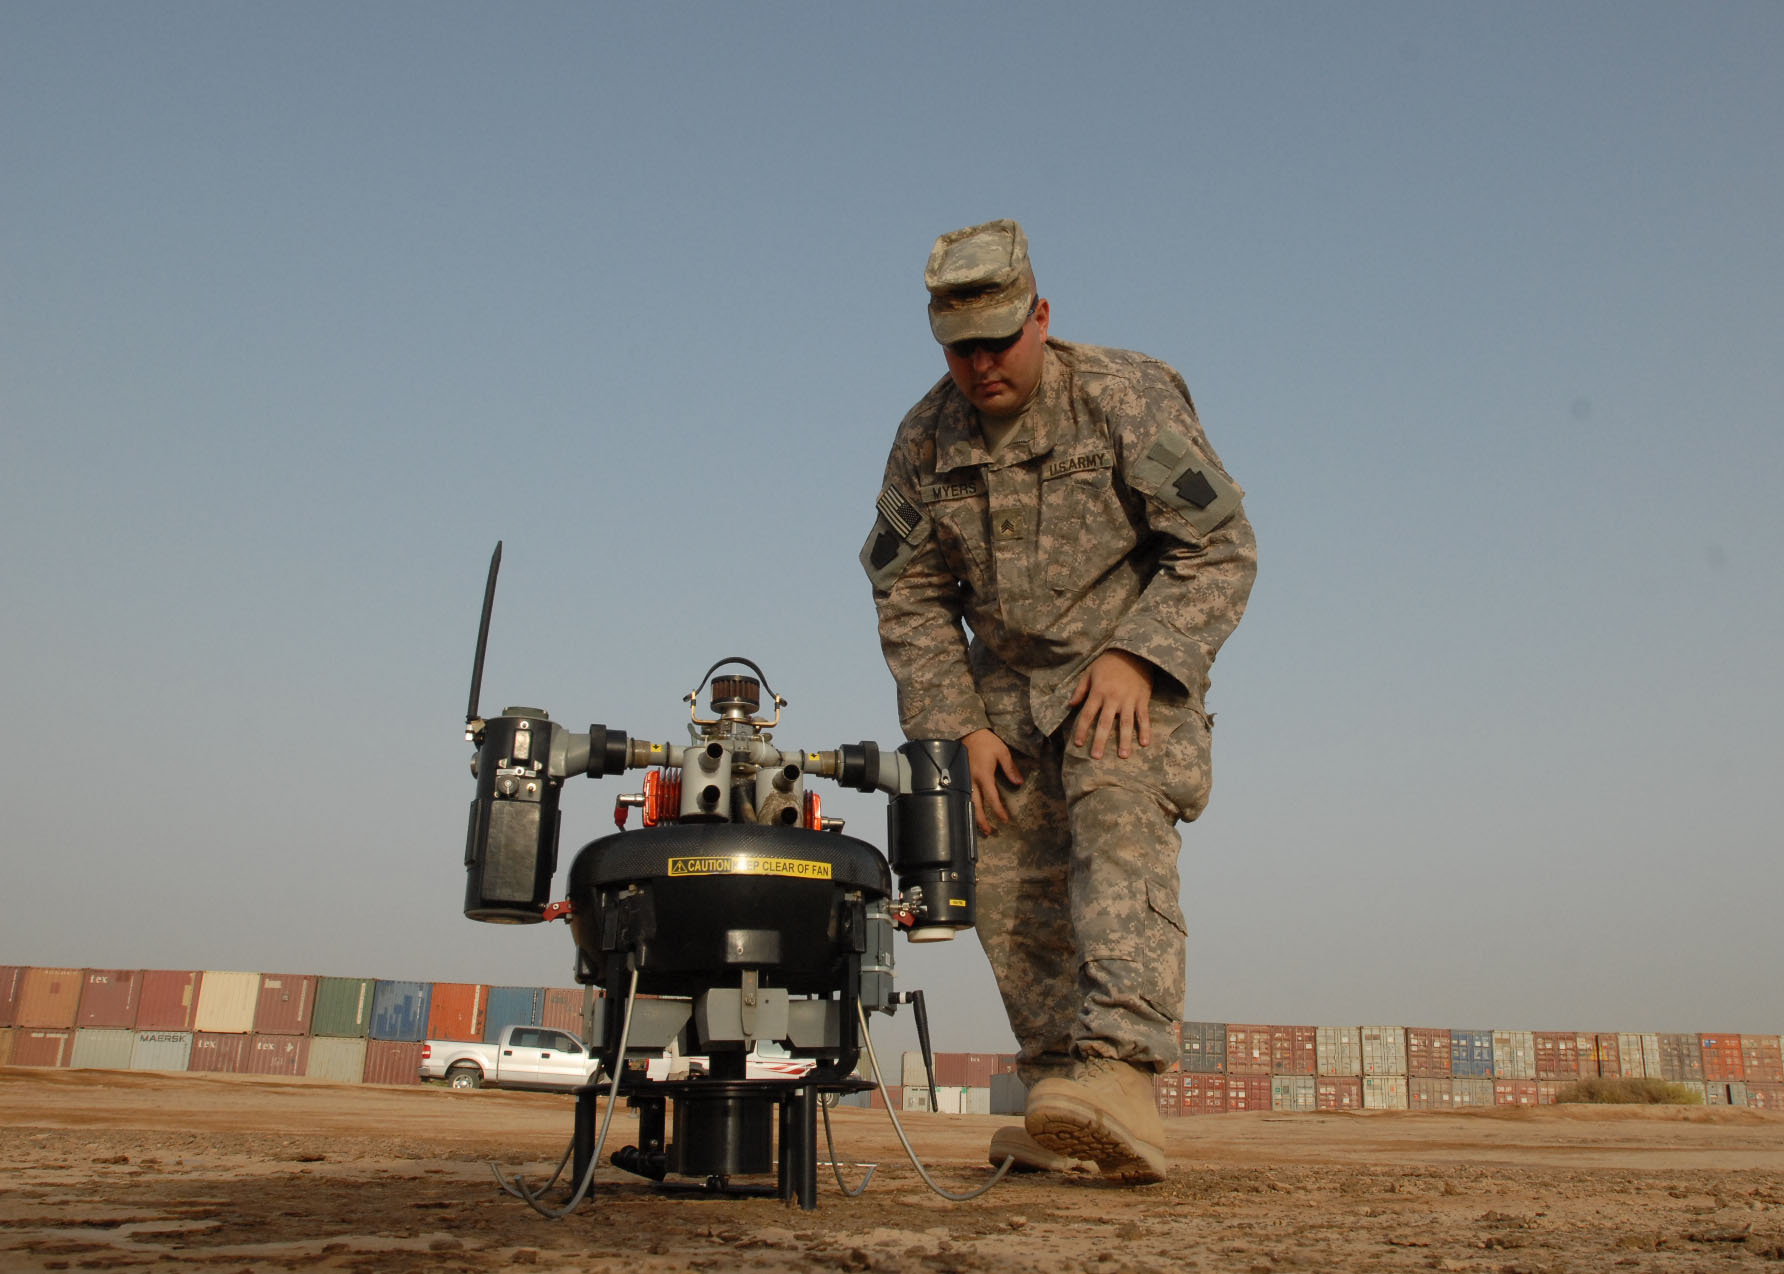
\includegraphics[width=4cm]{images/bitmap_image}
  \caption{Exemple d'image au format JPG.}
  \label{fig:une-autre-image}
\end{figure}


%%% Local Variables: 
%%% mode: latex
%%% TeX-master: "isae-report-template"
%%% End: 
\chapter{Une solution orientée BDD}
\label{chap:secondchapitre}

\section{Un DSL pour modéliser les exigences}

Nous avons montré dans la première partie la pertinence de la modélisation des exigences pour générer des tests fonctionnels. La modélisation qui répond au mieux à nos critères sont les DSL.  Nous avons vu que des outils comme Cucumber permettent à partir du DSL Gherkin ou encore EasyB, de passer des exigences à des tests.  Dans ces outils le DSL mis en place représente un scénario qui décrit un comportement du logiciel. Il s’agit donc d’une approche Behaviour Driven Developpement. Dans la solution que nous proposons, nous souhaitons garder ces éléments que nous pensons pertinents. Par conséquent, les personnes en charge de la rédaction des exigences devront se conformer au formalisme imposé par le DSL pour rédiger les exigences. Etant donné que le DSL représente un scénario qui est une modélisation connue des rédacteurs d'exigences et qui est une modélisation proche du langage naturel, nous pensons qu'il sera simple pour toutes les parties prenantes de lire et d'écrire les exigences dans ce format. 
Dans l'exemple que nous allons dérouler nous décidons de prendre comme DSL Gherkin et le langage Java pour l'implantation des méthodes mais la logique que nous proposons est tout à fait applicable à d'autres langages de programmation. Toutefois, il est possible qu'une entreprise souhaite développer son propre DSL car les spécificités de son domaine n'existent dans aucun DSL déjà programmé. Le nouveau DSL  devra imposer une structure qui permettra de déterminer quels sont les mots clés à partir desquels il faut générer une méthode de test. Dans le cas de Gherkin les termes "Scenario", "When", "And", "Given", "Then" du DSL permettent de générer une méthode de test à implanter. 

            \begin{figure}[H]
                \centering
                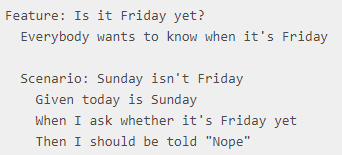
\includegraphics[width=\textwidth]{images/dsldsl.PNG}
                \caption{Exemple de scénario avec un DSL Gherkin}
            \end{figure}

\section{Génération des méthodes de test}

Une fois les exigences rédigées dans le DSL, pour chaque mot clé une signature de méthode est générée. Par exemple avec Cucumber : 

            \begin{figure}[H]
                \centering
                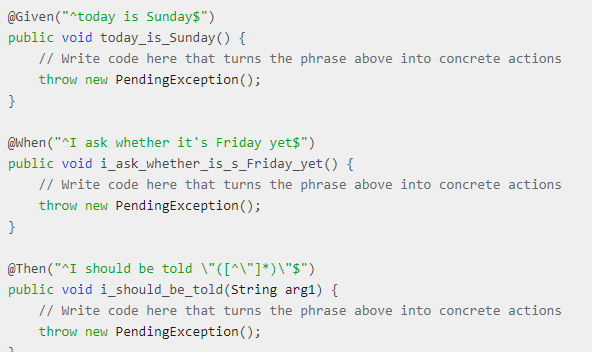
\includegraphics[width=\textwidth]{images/fixture.PNG}
                \caption{Exemple de méthodes de tests générés avec Cucumber}
            \end{figure}

Dans le corps de chaque méthode générée, un commentaire comme suit pour notifier que la méthode n'a pas encore été implantée :

\begin{lstlisting}
@Given("^today is Sunday$")
public void today_is_Sunday(){
// public void today_is_Sunday : TODO 
throw new PendingException();
}
\end{lstlisting}

D'autre part, nous souhaitons qu’à la génération de ces tests, un tableau de correspondance entre scénario, mot clé et signature générée soit automatiquement créé comme présenté dans la figure ci-dessous :

      \begin{table}[H]
        \centering
         \begin{tabular}{|c|c|c|c|c|} 
         \hline
        Scénario & Mot clé & Méthode de test associée & OK/KO/TODO \\ [0.5ex] 
         \hline
          & & \\
         \hline
        \end{tabular}
        \caption{Tableau généré à la suite de la définition des exigences}
        \end{table}
    
En prenant l'exemple des figures précédentes on aurait :

      \begin{table}[H]
        \centering
         \begin{tabular}{|c|c|c|c|c|} 
         \hline
        Scénario & Mot clé & Méthode de test associée & OK/KO/TODO \\ [0.5ex] 
         \hline
          Sunday isn't Friday & Given & public void today\_is\_Sunday() & \\
         \hline
         Sunday isn't Friday & When &  public void i\_ask\_whether\_is\_s\_Friday\_yet() & \\
         \hline
         Sunday isn't Friday & Then & public void i\_should\_be\_told()& \\
         \hline
        \end{tabular}
        \caption{Exemple de tableau de correspondance généré}
        \label{ref:correspondance}
        \end{table}
    
\section{Implantation des tests}

Les méthodes de tests avec le commentaire \textit{"\textcolor{dkgreen}{// signature de la méthode : TODO}"} devront être implantées par les développeurs. Quand une méthode est implantée, le commentaire \textit{"\textcolor{dkgreen}{"// signature de la méthode : TODO "} }devra impérativement être effacé par le développeur, sinon, la méthode sera considérée comme non développée. 

\section{Lancement des tests}

Les tests doivent pouvoir être lancés à n'importe quel moment du projet. Le résultat de chaque test devra être écrit en commentaire dans le corps de la méthode avec le format suivant : 
\begin{itemize}
    \item\textbf{signature de la méthode de test : OK si le test est passé }
    \item\textbf{signature de la méthode de test : KO si le test n'est pas passé.}
\end{itemize}


\begin{lstlisting}
@Given("^today is Sunday$")
public void today_is_Sunday(){
assert.equals("Test","Test")
// today_is_Sunday() : OK
throw new PendingException();
}
\end{lstlisting}

\section{Analyse des commentaires}

Une fois que les tests ont été lancés et les commentaires rédigés, nous proposons d'analyser ces derniers pour compléter le tableau \ref{ref:correspondance}. Pour chaque élément de la colonne \textit{"Méthode de test associée"}, les commentaires du code sont parcourus :
\begin{itemize}
    \item Si un commentaire (l'enchaînement de caractère \textbf{"\textcolor{dkgreen}{//}"} est détecté) est détecté et qu'il commence par le nom de la méthode associé, on lit ce qu'il y a après le caractère \textbf{"\textcolor{dkgreen}{:}"} et on le reporte dans le tableau dans la colonne \textit{"OK/KO/TODO"}.
    \item Si ce qu'il y a après le \textbf{"\textcolor{dkgreen}{:}"} est différent de \textbf{"OK","KO" ou "TODO", rien ne doit être reporté dans le tableau}
    \item Si la signature de la méthode n'est pas trouvée, rien ne doit être reporté et cela signifie qu'il y a un problème car une méthode présente doit être retrouvée dans le code. 
    \item Si deux commentaires \textit{"\textcolor{dkgreen}{"// signature de la méthode : TODO/KO/OK "}} sont présents dans le code, rien ne doit être insérer dans la colonne de resultat de test du tableau de correspondance car cela ne représente pas un comportement normal. 
\end{itemize}

A chaque lancement des tests, tous les commentaires de type \textit{"\textcolor{dkgreen}{"// signature de la méthode : OK "} } et \textit{"\textcolor{dkgreen}{"// signature de la méthode : KO "} } sont effacés. 

      \begin{table}[H]
        \centering
         \begin{tabular}{|c|c|c|c|c|} 
         \hline
        Scénario & Mot clé & Méthode de test associée & OK/KO/TODO \\ [0.5ex] 
         \hline
          Sunday isn't Friday & Given & public void today\_is\_Sunday() & OK\\
         \hline
         Sunday isn't Friday & When &  public void i\_ask\_whether\_is\_s\_Friday\_yet() & KO\\
         \hline
         Sunday isn't Friday & Then & public void i\_should\_be\_told()& TODO \\
         \hline
        \end{tabular}
        \caption{Tableau de correspondance après le lancement des tests}
        \end{table}
    
\section{Retour vers les exigences}

Nous souhaitons à présent remonter le résultat des tests au niveau des exigences pour que les personnes en charge de la recette puissent avoir une vision claire de quelles exigences ont été correctement implantées et lesquelles ne répondent toujours pas au besoin. Pour ceci, nous proposons de définir dans notre DSL des éléments graphiques de couleur pour chaque type de retour des tests. Ci-dessous la correspondance entre les messages de retour et les couleurs associées dans le DSL.

        \begin{table}[H]
        \centering
         \begin{tabular}{|c|c|} 
         \hline
        Retour & Couleur \\ [0.5ex] 
         \hline
          OK &  \cellcolor[HTML]{699A73}VERT\\
         \hline
          KO & \cellcolor[HTML]{D03737} ROUGE \\
         \hline
         TODO & \cellcolor[HTML]{4BB5C1}BLEU \\
         \hline
        \end{tabular}
        \caption{Correspondance du DSL entre retour des tests et couleurs}
        \end{table}

A la fin des tests, après le remplissage du tableau de correspondance \ref{ref:correspondance}, ce dernier est parcouru : 
Pour chaque scénario, et pour chaque mot clé, on dessine un triangle près du mot clé de la couleur correspondant au retour tel que défini dans la figure \ref{ref:colors}

            \begin{figure}[H]
                \centering
                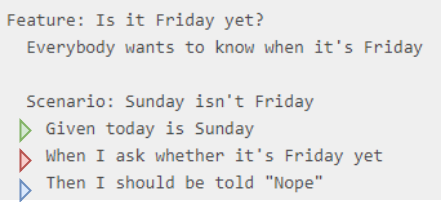
\includegraphics[width=\textwidth]{images/dslReturn.png}
                \caption{Retour des tests au niveau des exigences}
                \label{ref:colors}
            \end{figure}
            
Si le test n'a pas été trouvé, rien n'est affiché près du mot clé. Ainsi, toutes les parties prenantes ont une vision claire des exigences et peuvent en un lancement de test déterminer quelles exigences ont été respectées ou non.

\section{Critique de la solution}

Nous avons tenté de proposer une solution aux lacunes que d'autres outils possédaient. Toutefois, nous pensons que nous devons travailler sur quelques points pour l'améliorer.

Dans la solution proposée, les développeurs doivent manuellement effacer un commentaire de type \textit{TODO} dès qu'ils terminent d'implanter la méthode pour signifier que la méthode n'est plus à implanter. Leur donner le droit d'effacer un commentaire c'est aussi leur donner le droit d'en écrire. Un développeur peut écrire des assertions basiques pour tester une méthode. Par exemple, si un développement implante toutes les méthodes en écrivant :
\begin{lstlisting}
@Given("^today is Sunday$")
public void today_is_Sunday(){
assert.equals("Test","Test")
throw new PendingException();
}
\end{lstlisting}

Dans ce cas là toutes les méthodes retourneront un résultat OK à chaque lancement des tests. Donc toutes les notations graphiques seront au vert, ce qui fausse la réalité. Nous avons donc pas de moyen de vérifier la qualité de l'implantation du test. 


\chapter*{Conclusion}
\addcontentsline{toc}{chapter}{Conclusion}
\markboth{Conclusion}{Conclusion}
\label{chap:conclusion}



Dans ce mémoire nous nous sommes intéressés aux phases d'étude et de recette du cycle en V et de la méthode agile. Nous avons considéré que l'automatisation des tests d'acceptation à partir des exigences devait permettre à toutes les parties prenante de lire et/ou écrire les exigences, de générer automatiquement des tests fonctionnels et d'avoir un retour des tests au niveau des exigences. Nous avons montré que l'ingénierie des exigences pouvait être une piste intéressante pour répondre à notre problématique.

Nous avons d'abord présenté des outils qui permettaient de passer des exigences aux tests fonctionnels. Ceux-ci ne répondaient pas au critère d'automatisation. Nous avons ensuite, dans le cadre de l'ingénierie des exigences, proposé de modéliser les exigences dans un premier temps pour ensuite générer des tests fonctionnels à partir de cette modélisation. Des modélisations structurelles, comportementales ou encore des méthodes formelles ont été présentées. Ces modélisations étaient soit trop techniques, ou ne présentaient pas assez de détails ou encore ne permettaient pas de générer des tests. Toutefois, nous avons vu que les Domain Specific Language permettaient de réunir bon nombre de nos critères notamment le critère d'impliquer le domaine métier au coeur de la modélisation, de proposer une simplicité d'écriture et de lecture pour toutes les parties prenantes et surtout la génération des tests fonctionnels. Par conséquent, nous nous sommes tournés vers les outils orientés Behaviour Driven Developement tel que Cucumber qui propose un DSL représentant des scénarios à partir desquels des signatures de méthodes de tests fonctionnels sont générés. Néanmoins, ce genre d'outils ne permettant pas d'avoir un retour clair au niveau des exigences du résultat des tests, nous avons souhaité proposer notre propre solution.

Pour tenter de répondre à tous les critères que nous avions établi, nous avons proposer de mettre en place un outil basé sur un DSL pour représenter les exigences à partir duquel les tests d'acceptation seraient générés grâce à des mots clé définis. Une fois ces tests implantés par les développeurs, à chaque fois qu'ils sont testés, des commentaires qui décrivent le résultat de chaque test sont rédigés dans le code. Les commentaires sont ensuite analysés : si le test est passé un élément graphique coloré, défini dans le DSL s'affichera près de chaque mot clé pour signifier le résultat du test. Ainsi, quelque soit la partie prenante, il est possible de savoir quelle exigence a été respectée ou non en un coup d'oeil.
Cependant notre solution présente des failles, notamment de qualité, car les développeurs peuvent influencer manuellement le résultat des tests. 
Il serait intéressant, après avoir pallié à ces failles, d'étendre cette solution à d'autres types de tests tels que des test non-fonctionnels ou de contrainte par exemple.
\appendix

\bibliographystyle{authoryear-fr}
\bibliography{references}


\end{document}
